\documentclass{article}

\usepackage{graphicx} 
\usepackage{subfigure}
\usepackage{paralist}

\usepackage{hyperref}

\usepackage{url}
\usepackage{booktabs}

\usepackage[usenames,dvipsnames]{xcolor}
\usepackage{tikz}
\usetikzlibrary{positioning, calc}

\usepackage[draft,nomargin,footnote]{fixme}

\graphicspath{{figs/}}

\usepackage{xspace}
\newcommand{\eg}{\textit{e.g.}\xspace}
\newcommand{\etal}{\textit{et al.}\xspace}
\newcommand{\ie}{\textit{i.e.}\xspace}
\newcommand{\etc}{\textit{etc.}\xspace}
\newcommand{\vs}{\textit{vs.}\xspace}

\title{Learning by Teaching a Robot: the Case of Handwriting}

\author{S\'everin Lemaignan$^1$, Alexis Jacq$^{1,2}$, Fernando Garcia$^1$,
    Deanna Hood$^1$, \\Aude
    Billard$^1$, Ana Paiva$^2$, Pierre Dillenbourg$^1$ \\
$^1$CHILI Lab, \'Ecole Polytechnique F\'ed\'erale de Lausanne, Suisse,\\
$^2$Instituto Superior T\'{e}cnico, University of Lisbon, Portugal}

\begin{document}
\maketitle

\begin{abstract}

    Robots for education are not limited to support ICT teaching, and robots are
    finding new ways to enter and blend in the classroom. This article reports
    on such a new paradigm for educative robots, that involves \emph{learning by
    teaching} and strong \emph{social engagement} to help children struggling
    with handwriting. Our system relies on machine-learning and child-robot
    interaction with a small humanoid robot, and we present several real-world
    studies in schools and with occupational therapists that led us to promising
    initial results.

\end{abstract}


%%%%%%%%%%%%%%%%%%%%%%%%%%%%%%%%%%%%%%%%%%%%%%%%%%%%%%%%%%%%%%%%%%%%%%%%%%%%%%%%%%%
%%%%%%%%%%%%%%%%%%%%%%%%%%%%%%%%%%%%%%%%%%%%%%%%%%%%%%%%%%%%%%%%%%%%%%%%%%%%%%%%%%%
%%%%%%%%%%%%%%%%%%%%%%%%%%%%%%%%%%%%%%%%%%%%%%%%%%%%%%%%%%%%%%%%%%%%%%%%%%%%%%%%%%%
\section{A Different Paradigm for Educative Robots}

Henry is five and an half, and has been diagnosed with visuo-constructive
deficits. He is under the care of an occupational therapist, and tries to
workaround his inability to draw letters in a consistent manner. Diego is six
and struggles at school with his poor handwriting and even poorer
self-confidence.

While Henry is lively and always quick at shifting his attention from one
activity to another, Diego is shy and poised. Two very different children,
facing however the same difficulty to write in a legible manner. And, hidden
beyond this impaired skill, psycho-social difficulties also arise: they
underperform at school, Henry has to go for follow-up visits every week,...
they live under the label ``requires special care''. This is a source of
anxiety, for the children, and for their parents alike.

\begin{figure}
    \centering
    \includegraphics[width=0.9\linewidth]{henry}
    \caption{\small Henry teaching Nao how to write numbers, with the help of an
    occupational therapist.}
    \label{fig:henry}
\end{figure}

Remediations for handwriting difficulties traditionally involve long
interventions (at least 10 weeks, \cite{Hoy2011}), essentially consisting in
handwriting training with occupational therapists, and primarily addressing the
\emph{motor} deficits.  Improvements in self-confidence and anxiety occur (at
best) as a side-effect of the child improving his/her handwriting skills and,
consequently, improving his/her performance at school.

We present in this article a new take on this educative challenge, as a
remediation procedure that involve a \emph{bad writer} robot that is taught by the
child: by building on the \emph{learning by teaching} paradigm, not only the
child practises hand-writing but, as (s)he takes on the role of the teacher,
(s)he also positively reinforce his/her self-esteem and motivation: his/her
social role shifts from the ``underperformer'' to ``the one who knows and teaches''.

\subsection{Learning by Teaching}

The \emph{learning by teaching} paradigm, which engages the student in the act
of teaching another, has been shown to produce motivational, meta-cognitive, and
educational benefits in a range of disciplines~\cite{Rohrbeck2003}.  The
application of this paradigm to handwriting intervention remains, however,
unexplored. One reason for this may be due to the requirement of an
appropriately unskilled peer for the child to tutor: it may prove difficult if
the child is the lowest performer in his/her class.  In some cases, it may be
appropriate for a peer or teacher to simulate a na\"ive learner for the target
child to teach. For handwriting however, where one's skill level is visually
evident, this acting is likely to be rapidly detected. This motivates the use of
an artificial teachable agent which can be configured for a variety of skill
levels, and for which children do not have preconceptions about its handwriting
ability.

Robots have been used as teachers or social partners to promote children's
learning in a range of contexts, most commonly related to language
skills~\cite{han2010robot}, and less often to physical skills (such as
calligraphy~\cite{Matsui2013}). Looking at the converse (humans \emph{teaching}
robots), Werfel notes in~\cite{Werfel2014} that most of the work focuses on the
robot's benefits (in terms of language~\cite{Saunders2010} or
physical~\cite{Mulling2013} skills, for example) rather than the learning
experienced by the human tutor themselves.  Our work concentrates on this latter
aspect: by demonstrating handwriting to a robot, we aim at improving the
\emph{child's} performance. Note that our work must be distinguished from
``learning from demonstration'' approaches to robots learning physical skills,
as the agent we present is only simulating fine motor skills for interaction
purposes.

A robotic learning agent which employs the learning by teaching paradigm has
previously been developed by Tanaka and Matsuzoe~\cite{Tanaka2012}. In their
system, children learn vocabulary by teaching the {\sc nao} robot to act out
verbs. The robot is tele-operated (Wizard-Of-Oz) and mimics the actions that the
children teach it, but with no long-term memory or learning algorithm in place.
Our project significantly extends this line of work in two ways. First, by
investigating the context of children's acquisition of a challenging physical
skill (handwriting), and second by proposing a robotic partner which is fully
autonomous in its learning.

\subsection{Agency and Commitment}

The work presented here investigates a particular role for a robot in the
education of handwriting: not only is the robot actively performing the activity
by drawing letters, but it does so in a way that engages the child in a very
specific social role. The child is the teacher in this relationship and the
robot is the learner: the child must engage in a (meta-) cognitive relationship
with the robot to try to understand why the robot fails and how to help it best.
Here, the robot is more than just an activity facilitator or orchestrator -- its
physical presence and embodiment induce agency and anthropomorphising, and
cognitively engage the child into the learning activity.

Besides that, the commitment of the child into the interaction build on the
``protégé effect'': teachable computer-based agents have previously been used to
encourage the ``protégé effect'', wherein students invest more effort into
learning when it is for a teachable agent than for themselves~\cite{Chase2009}.
As we are concerned with learning of a physical skill, the learning agent
developed is embodied in a humanoid robot which is capable of physically
demonstrating handwriting trajectories to its child learning partner.  This is
supported by the potential for motor mimicry to yield significant improvements
in handwriting interventions in which letter formations are demonstrated to
participants~\cite{Berninger1997}. Furthermore, when compared to screen-based
agents, robotic partners have been shown in some contexts to increase users'
compliance with tasks~\cite{Bainbridge2011}, maintain more effective long-term
relationships~\cite{Kidd2008}, and produce greater learning gains when acting as
tutors~\cite{Leyzberg2012}.

For these two reasons, our approach is to be distinguished from previous works in
educational robotic. Most of these do not consider the agency induced by the
robot beyond its motivational aspect: playing with an interactive, partially autonomous
device naturally induces some form of anthropomorphizing, which leads to some
level of projected agency, and participate the overall excitement (at least, on
the short-term, before the novelty effect vanishes).

In our case, the role of agency is stronger: it induces meta-cognition (``I am
interacting with an agent, so I need to reflect on how to best teach him''),
which is beneficial for the learning process; it also induces a protégé effect
(``I want my robot-agent to succeed!'') which support the commitment of child
into the interaction, also for longer period of time (we report in this article
upon to case studies where children were interacting with the same robot for several
hours, spanned over several weeks).

\subsection*{Overview of the article}

We have sofar frame our intents: to design a robotic system that would support
handwriting remediation in an original way: by getting children to teach a
robotic agent how to write, those children would both practise without knowing
it and recover self-confidence and self-esteem by supporting a
worst-than-themselves robotic ``student''.

The following sections of the paper go into details. The next section provides a
brief overview of the robotic system and the interaction it induces. We then
give the details of machine-learning techniques that allow the robot to learn
from the children, followed by the implementation on the Nao robot.

Next, we present and report on the four school experiments and the two case
studies that we conducted over the last two years. While the focus of the school
experiments was mostly technical validation and data acquisition, the two case
studies that lasted each about 4 weeks, gave us initial insights on the
relevance and effectiveness of our approach.

%%%%%%%%%%%%%%%%%%%%%%%%%%%%%%%%%%%%%%%%%%%%%%%%%%%%%%%%%%%%%%%%%%%%%%%%%%%%%%%%%%%
%%%%%%%%%%%%%%%%%%%%%%%%%%%%%%%%%%%%%%%%%%%%%%%%%%%%%%%%%%%%%%%%%%%%%%%%%%%%%%%%%%%
%%%%%%%%%%%%%%%%%%%%%%%%%%%%%%%%%%%%%%%%%%%%%%%%%%%%%%%%%%%%%%%%%%%%%%%%%%%%%%%%%%%
\section{Implementation of the Interaction}

Figure~\ref{experimental_setup} illustrates our general experimental setup: a
face-to-face child-robot interaction with an (autonomous) Aldebran's Nao robot.

A tactile tablet (with a custom application) is used for both the robot and the
child to write: during a typical round, the child requests the robot to write
something (a single letter, a number or a full word), and push the tablet
towards the robot, the robot writes on the tablet by gesturing the writing, but
\emph{without actually physically touching the tablet}), the child then pull
back the tablet, correct the robot's attempt by writing him/herself on top or
next to the robot's writing (see the picture in Figure~\ref{fig:diego}), and
``send'' his/her demonstration to the robot by pressing a small button on the
tablet. The robot ``learns'' from this demonstration and tries again.

Since the child is assumed to take on the role of the teacher, we had to ensure
(s)he would be able to manage by him/herself the turn-taking and the overall
progression of the activity (moving to the next letter or word). In our design,
the turn-taking relies on the robot prompting for feedback once it is done with
its writing (simple sentences like ``What do you think?''), and pressing on a
small robot icon on the tablet once the child has finished correcting. In our
experiments, both were easy to grasp for children.


\begin{figure}
    \centering
    
\includegraphics[width=0.6\columnwidth]{experimental_setup}
    \caption{\small Our experimental setup: face-to-face interaction with a {\sc
        nao} robot.  The robot writes on the tactile tablet, the child then
        corrects the robot by directly overwriting its letters on the tablet
        with a stylus. An adult (either a therapist or an experimenter,
        depending on the studies), remains next to the child to guide the work
        (prompting, turn taking, etc.). For some studies, a second tablet and an
        additional camera (dashed) are employed.}

    \label{experimental_setup}
\end{figure}

Implementing such a system raises several challenges: first, acquiring,
analyzing and learning from hand-written demonstration lays at the core of the
our approach and we developed several algorithms for the robot to generate
initial bad writing and to respond in an adequate manner, showing visible (but
not too quick) writing improvements.

Then, the actual implementation on the robot required the coordination of
several modules (from performing gestures and acquiring the user's input to
the high-level state machine), spread over several devices (the robot itself,
one laptop and up to four tactile tablets for certain studies we conducted). We
relied on ROS to ensure the synchronization and communication between these
modules.

We detail each of these in the following sections.

%%%%%%%%%%%%%%%%%%%%%%%%%%%%%%%%%%%%%%%%%%%%%%%%%%%%%%%%%%%%%%%%%%%%%%%%%%%%%%%%%%%
\subsection{Generating and Learning Letters}

Since our application is about teaching a robot to write, generating (initially
bad) letters and learning from demonstrations is a core aspect of the project.

The main insight for both the generation and the learning of letters is to
reason in the eigenspace of the letters, instead of the cartesian space. The
eigenspace of each letters is spanned by the first $n$ eigenvectors (in our
experiments, $3 < n < 6$) of the covariance matrix observed in a standard
dataset of adult letters (the UJI Pen Characters 2 dataset~\cite{Llorens2008}).
This procedure, based on a Principle Component Analysis (PCA), is explained in
details in a previously published article~\cite{hood2015when}.

By changing the eigenvalues associated to these eigenvectors and regenerating
letters with the reverse procedure, it becomes then easy to generate new
letters, with distortions that are actually plausible handwriting errors: they
are actually \emph{exaggerations} of variance of writing styles that naturally
exist amongst adult writers.  Figure~\ref{fig:sampleLetters} shows examples of
deformed ``g'' generated with such a technique.

\begin{figure}
    \centering
    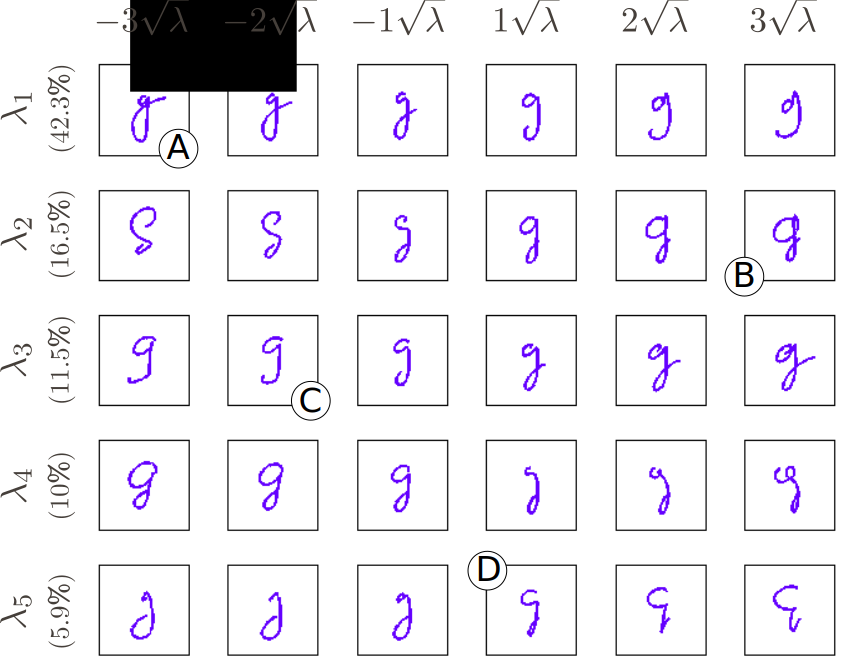
\includegraphics[width=0.9\linewidth]{cowriter-g}
    \caption{\small \label{fig:sampleLetters} \textbf{Generating bad letters}:
        effect of varying the first five eigenvalues (rows) of the shape model
        of ``g'' by different factors (columns). The percentage of the total
        variance in the dataset explained by each eigenvalue is shown      on
        the appropriate row. Examples noted A, B, C, D illustrate how the
        PCA-based approach allows to \emph{automatically} generate letters whose
        errors can be \emph{semantically} interpreted: A has a too large bottom
        loop, B has a wide top loop, the bottom loop of C is not correctly
        closed, the top loop of D is not closed.}

\end{figure}

The same technique can be applied to \emph{classify} demonstrations,
\emph{assess} their quality and
\emph{learn} from them. Figure~\ref{fig:h} shows 9 allographs of ``h'' written by a 6
years old child, along with the mean letter from the
dataset (reference letter). By projecting each of the demonstrations onto the eigenspace
of ``h'' (Figure~\ref{fig:h}b), we observe that:

\begin{itemize}
    \item the different allographs can by clustered (with a $k$-means or
        mean-shift algorithm) by their visual styles,
    \item we can compute an euclidian distance to the reference letter to assess
        the visual proximity of the demonstration with the expected letter, thus
        providing a quantitative metric of writing performance.
\end{itemize}

\begin{figure}[ht!]
    \centering
    \subfigure[Nine allographs of the cursive ``h'', next to the reference]{
        \includegraphics[height=4.1cm]{h}
    }
    \subfigure[Same samples, normalized and projected in the eigen space spanned from the
        3 first eigenvectors: clusters arise, that actually match writing styles.]{
        \includegraphics[height=4.5cm]{eigenspace-uniformization}
    }

    \caption{\small Projecting demonstrated letters onto the eigenspace
    generated from the reference dataset effectively clusters the samples
    according to their topological similarity. Allographs that are visually similar to
    the reference are close to it in the eigenspace.}
    \label{fig:h}
\end{figure}

The algorithm for machine-learning becomes then a simple matter of converging at
a specific pace towards the child demonstration in the eigenspace.
Figure~\ref{learning_6_demos}, at the end of the article, shows a complete learning cycle
with the number ``6''.

%%%%%%%%%%%%%%%%%%%%%%%%%%%%%%%%%%%%%%%%%%%%%%%%%%%%%%%%%%%%%%%%%%%%%%%%%%%%%%%%%%%
\subsection{Robotic Implementation}

Our system is embodied through an Aldebaran's {\sc nao} (V4 or V5, depending on the studies)
humanoid robot. This choice is motivated by its approachable
design~\cite{Gouaillier2008}, its size (58cm) and inherently safe structure (lightweight
plastic) (making it suitable for close interaction with children), its low price
(making it closer to what school may afford in the coming years) and finally its
ease of deployment on the field.

{\sc nao} is a humanoid biped, has 25 degrees of freedom,
two cameras, speech capabilities and the ability to autonomously execute a range
of tasks. While it can walk, this capability is not used in this project, and
the robot remains in a crouching posture during the whole interaction.

Robotic handwriting requires precise closed-loop control of the arm and hand
motion. Because of the limited fine motor skills possible
with such an affordable robot, in addition to the absence of force feedback and
other technical necessities, we have opted for \emph{simulated
handwriting}: the robot draws letters in the air, and the actual writing is
displayed on a synchronised tablet.

\begin{figure}[ht!]
\centering

\resizebox{0.6\linewidth}{!}{%

\begin{tikzpicture}[
    >=latex,
    node distance=2cm,
    every edge/.style={draw, very thick},
    redarrow/.style={draw,red, text=black},
    greenarrow/.style={draw,GreenYellow,text=black},
    yellowarrow/.style={draw,BurntOrange,text=black},
    cmpt/.style={draw, align=center, rounded corners, inner sep=5pt, font=\sf, fill=black!20},
    label/.style={midway, align=left, font=\scriptsize\sf, fill=white, above,opacity=0,text opacity=1}]

    \node at (0,0) (laptop) {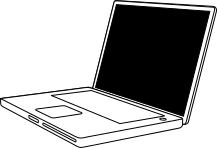
\includegraphics[width=2cm]{laptop}};
    \node[below right=2 of laptop] (nao) {
\includegraphics[width=2cm]{nao}};
    \node[below left=2 of laptop] (tablet) {
\includegraphics[width=2cm]{tablet+stylus}};
    \node[above=2 of laptop] (selection) {
\includegraphics[width=2cm]{selection_tablet}};

    \path (nao) edge [->,redarrow, bend left] node[label, auto] {robot state} (laptop);
    \path (laptop) edge [->,greenarrow, bend left] node[label, auto] {writing gesture} (nao);

    \path (tablet) edge [->,redarrow, bend left] node[label, auto] {demonstrations,\\turn taking} (laptop);
    \path (laptop) edge [->,redarrow, bend left] node[label, auto=right] {letter to write} (tablet);

    \path (selection) edge [->,redarrow] node[label, auto] {letter/word to write} (laptop);

    \path (-5, 2) edge [->, redarrow] node[label] {ROS} ++(1, 0);
    \path (-5, 2.6) edge [->, greenarrow] node[label] {NaoQI} ++(1, 0);
    
\end{tikzpicture}
}

\caption{\small Overview of the system. In total, the system runs about 10 ROS nodes,
    distributed over the robot itself, a central laptop and Android tablets.}

    \label{fig:archi}
\end{figure}

The overall architecture of the system (Figure~\ref{fig:archi}) is therefore
spread over several devices: the {\sc nao} robot itself, that we address via
both a ROS API\footnote{The ROS stack for {\sc nao} is available at
\url{http://wiki.ros.org/nao_robot}.} and the Aldebaran-provided NaoQI API, one
to four Android tablets (the main tablet is used to print the robot's letter and
to acquire the children's demonstrations. More tablets have been used in some
studies, either to let the child input words to be written, or for the
experimenter to qualitatively annotate the interaction in a synchronized
fashion), and a central laptop running the machine learning algorithms, the
robot's handwriting gesture generation and high level control of the activity.

Since the system does not actually require any CPU-intensive process, the laptop
could be removed and the whole logic could run on the robot. Due to the relative
difficulty to deploy and debug ROS nodes directly on the robot, we however
effectively kept the laptop during our experiments.

Most of the nodes are written in Python, and the whole source code of the
project is available online\footnote{The primary repository is
\url{https://github.com/chili-epfl/cowriter_letter_learning}.}

\subsubsection*{Trajectory Following Movements}

Using simulated handwriting provides an opportunity for the robot's writing to
appear smoother than would be achievable with a writing instrument. However, the
robot's motions must still sufficiently match the displayed trajectory in order
capture the engagement of the child participant in the action. Aldebaran's NaoQi
API is used for the inverse kinematics of the trajectory following. ROS is used
for integration of {\sc nao} with external reference frames, such as the
tablet's location, using the $tf$ transformation library~\cite{Foote2013}.

When using simulated handwriting, it is no longer necessary that the robot
engages in the typical style of handwriting of using a writing instrument at a
desk. Having instead the robot point at the writing surface to cause the
trajectory to appear (as seen in Figure \ref{fig:schools}, left) has several advantages:

\begin{itemize}

    \item The working space of the robot increases, both in the technical sense
        and the interaction sense: someone can, in theory, show the tablet to
        the robot from across the room and have it still respond, without
        needing the tablet to be within arm's reach,

    \item Concerns about whether or not the child would start mimicking the
        robot's incorrect writing form (\eg pen grip) are mitigated,

    \item Perhaps most significantly, the accuracy of the matching of the
        robot's motion with the trajectory displayed on the tablet is not as
        critical. This is because a pen tip would be expected to touch the
        tablet exactly at the trajectory point, while a fingertip may not.

\end{itemize}

We have therefore designed the system in such a way that the robot is simulating
handwriting by pointing at the tablet\footnote{Teachers interviewed for their
feedback on the system advised that children are asked to draw letters in
the air in a similar manner as part of their handwriting education. The
behaviour is hence not unfamiliar to children.}. As interacting with a
tablet with one's finger is not uncommon, this may aid the acceptance of the
writing style by users. 

Because motion planning is performed with respect to the hand of the robot,
rather than its fingertip, one or two of the orientation degrees of freedom of
the hand are fixed to keep the finger approximately perpendicular to the writing
surface, depending on the desired accuracy. The remaining free orientation(s),
coupled with the whole-body motion control available, allow for a sufficient
working space for writing on the entire tablet.



%%%%%%%%%%%%%%%%%%%%%%%%%%%%%%%%%%%%%%%%%%%%%%%%%%%%%%%%%%%%%%%%%%%%%%%%%%%%%%%%%%%
%%%%%%%%%%%%%%%%%%%%%%%%%%%%%%%%%%%%%%%%%%%%%%%%%%%%%%%%%%%%%%%%%%%%%%%%%%%%%%%%%%%
%%%%%%%%%%%%%%%%%%%%%%%%%%%%%%%%%%%%%%%%%%%%%%%%%%%%%%%%%%%%%%%%%%%%%%%%%%%%%%%%%%%
\section{Field Studies}

To date, the presented system has been deployed and tested in three different
schools (totalling child-robot interactions with more than 70 children, aged 5
to 8) and we also conducted 2 case studies over several weeks.
Table~\ref{studies} gives an overview of these studies.

\begin{table}[ht!]
\centering
\caption{\small Field studies conducted within the project}
\label{studies}
\begin{tabular}{@{}lp{4.5cm}p{2.2cm}p{2.5cm}l@{}}
\toprule
{\bf Study}     & {\bf Type}                                    & {\bf Duration}              & {\bf Children \#}                     & {\bf Ages} \\ \midrule
{\it ISG 1}     & Unstructured group interaction at school      & 16 min/group               & 4 $\times$ 8 children                 & 6-7        \\
{\it Florimont} & Individual/Pair interaction at school         & 11 min/group               & 7 (individual) + 7 $\times$ 2 (pairs) & 7-8        \\
{\it Diego}     & Case-study, spanning over 4 weeks              & 1.5 hours $\times$ 4 weeks & 1                                     & 5          \\
{\it Haut-Lac}  & Pair (with turn-taking) interaction at school & 26 min/group                            & 7 $\times$ 2                          & 5-6        \\
{\it ISG 2}     & Individual interaction at school              & 18 min                            & 6                                     & 5-6        \\
{\it Henry}     & Case-study, spanning over 4 weeks              & 1h $\times$ 4 weeks        & 1                                     & 5          \\ \bottomrule
\end{tabular}
\end{table}

%%%%%%%%%%%%%%%%%%%%%%%%%%%%%%%%%%%%%%%%%%%%%%%%%%%%%%%%%%%%%%%%%%%%%%%%%%%%%%%%%%%
\subsection{Studies at School}

Over the two years of the project, we conducted four studies in schools
(Figure~\ref{fig:schools}). These experiments were meant to technically validate
the system (is it actually able to autonomously write and learn from
demonstrations?) and the interaction (is the apparatus easy to grasp and to
interact with for children), and to study the initial acceptance of the robot in
the school environment (we conducted several formal and informal discussions
with teachers).

We also relied on these four studies to acquire a dataset of children's
handwritten letters and to study how they engage with the robot (and maintain or
not this engagement).

\begin{figure}
    \centering
    \includegraphics[height=3.9cm]{schools}
    \includegraphics[height=3.9cm]{schools2}
    \caption{\small The first field studies were focused on technical validation, with
    above 70 pupils interacting with the robot over short periods (around 15
minutes), either alone or in small groups.}
    \label{fig:schools}
\end{figure}

Critically, these studies were conducted with \emph{whole classes}: we did not
select underperforming children that requires careful beforehand organization
with the school to limit ethical issues. Having more children (73 in total) was
however beneficial for these preliminary studies.

\paragraph{System validation}

From a technical perspective, the system achieves an acceptable level of
reliability and allow a technically sound autonomous interaction. For instance,
during the second school study (\textit{Florimont}), the robot withstood
interactions which lasted for a total of 160 minutes.  During this time the
robot wrote 335 letters, 152 of which in response to demonstrations received
from the 21 children. Technical intervention was only required for the three
instances that the robot fell later in that day.  Otherwise, the technical
components of the system operated autonomously and as expected over the
sessions.

Due to the modular software architecture (about 10 ROS nodes), crashes occurring
during the sessions were usually quickly resolved by re-launching the faulty
node alone, and did not significantly impact the interaction.

The otherwise technical limitations were related to some letters or writing
style (most notably, the ones requiring multiple strokes per letter) not being
adequately processed by the learning algorithm. Support for such letters has
been since added.

\paragraph{Acceptance}

For the approach to be effective, it is critical that children recognize and
accept that the robot is writing by itself. When asked, no child indicated that
they did not believe that the robot was writing by itself. There were, at times,
questions about the robot's writing method at the beginning of the interaction,
but when advised that the robot ``tells the tablet what it wants to write,''
this was accepted by the children.  Besides, teachers interviewed for their
feedback on the system advised that children are asked to draw letters in the
air in a similar manner as part of their handwriting education. The behaviour is
hence not unfamiliar to children.

\paragraph{Engagement}

As indicated in the introduction, literature~\cite{Hoy2011} suggests that a
total of 20 handwriting practice sessions is found to be the minimum to demonstrate effective
results in handwriting remediation. This highlights the necessity to sustain
engagement over the long-term if we want to achieve measurable learning gains.

Factually, the children engaged into the teaching activity: in the
\textit{Florimont} study, for instance, they demonstrated an average of
10.9 demonstration letters (SD = 4.4) for an average session duration of 11 minutes.
In 9 out of the 14 sessions (64\%), the robot
received demonstration letters even \emph{after} reaching the final stage of the
interaction, suggesting an intrinsic motivation to further engage in the
interaction.

\begin{figure}[ht!]
    \centering
    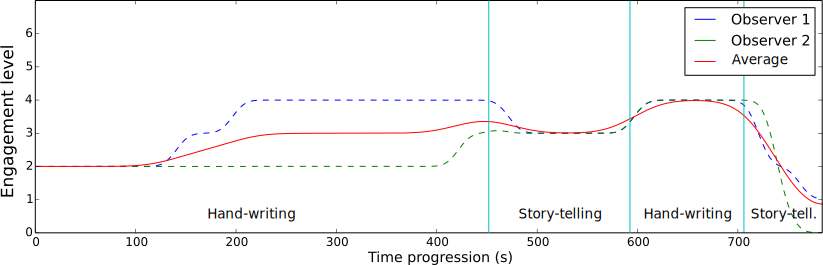
\includegraphics[width=0.9\linewidth]{engagement}
    \caption{Engagement level of one child, manually annotated by two judges
        over a 13 min long interaction (Cronbach’s alpha test: $\alpha = .82$,
        good inter-judge agreement). 0 means ``complete disengagement from the
        task'', 6 means ``full engagement''. The vertical lines represent activity
    switches between handwriting teaching and story-telling (used as a
    distruber).}
    \label{engagement_level}
\end{figure}

We also conducted a qualitative assessment of the engagement levels during the
interaction sessions (studies \textit{Haut-Lac} and \textit{ISG 2}).
Figure~\ref{engagement_level} shows the result for one child, with a moderate
level of engagement. On-going research in our group aims at assessing such
engagement levels in real-time, and adapt accordingly its behaviour.

Other qualitative assessment of engagement over longer interactions were
conducted during the case studies, as reported in the following section.

%%%%%%%%%%%%%%%%%%%%%%%%%%%%%%%%%%%%%%%%%%%%%%%%%%%%%%%%%%%%%%%%%%%%%%%%%%%%%%%%%%%
\subsection{Case Study 1: Diego}

\subsubsection{Context, Study Design}
It was the first time we where trying a long-term interaction between a child
and the CoWriter robot. So the first aim of this study was to see if such an
interaction was simply possible. If we could create an environment to keep a child engaged
during one hour just in writing words with the robot.
The second question was focused on the content of the interaction. Our goal was
to figure out what extent the child would actually improve the robot's
writing.\\

Diego is a six years old child. 
Before the experiment, we could create a dataset of letters based on his main
mistakes, but amplified by PCA. Our idea was to make the robot
exaggerating the mistakes of Diego. Thus, by correcting the robot, 
Diego was actually going to correct himself.\\

The experiment took one month. It was divided in four sessions of one hour, one session per week.
In order to justify to the child an activity where a robot wants to learn
handwriting, we decided to adduce a scenario. There where two Nao robots: a
blue one (Mimi) and an orange one (Clem). They where introduced to the child as
two hold friends. Mimi was left, and the two robots were corresponding by
handwritten mails. But Clem was beginning in writing and it needed the help of
Diego to write its responses to Mimi.\\

During the first session, Diego was just teaching single letters to the robot.
Gradually we increased the difficulty : the second session he was teaching
shirt words and in third session he was teaching long sentences. The last session was more like a test for Clem
: it had to prove to Mimi that it actually improved its handwriting thanks to
Diego. 


\begin{figure}
    \centering
    \includegraphics[width=0.5\linewidth]{diego}
    \caption{\small Diego working with Nao}
    \label{fig:diego}
\end{figure}


\subsubsection{Results}
Diego completely accepted our scenario and seriously played the game. At the
beginning he seemed not confident and intimidated.  But quickly, he gain in
confidence and complicity with the robot. Finally, he showed a real affinity, so
that he sent an handwritten mail to it some days after the last
session.\\ 

In all sessions, Diego was fully focused on the activity during forty minutes up to one
hour. In total, he provided 154 letters as demonstration.\\

Diego felt he improved the robot's handwriting. To make clearly visible this
improvement, we printed the letter that the robot wrote during the third
session before and after the help of Diego~\ref{fig:stimuli}.


\begin{figure}
    \centering
    \subfigure[Initial letter, generated by the robot]{
        \includegraphics[height=6cm]{diego-initial-letter}
    }
    \subfigure[Final letter, after training with Diego]{
        \includegraphics[height=6cm]{diego-final-letter}
    }

    \caption{\small Text generated by the robot, before and after training with
    the child. As an example, the red box emphasizes the changes on the word
    ``envoyer''.}
    \label{fig:stimuli}
\end{figure}


%%%%%%%%%%%%%%%%%%%%%%%%%%%%%%%%%%%%%%%%%%%%%%%%%%%%%%%%%%%%%%%%%%%%%%%%%%%%%%%%%%%
\subsection{Case Study 2: Henry}

\subsubsection{Context, Study Design}
Henry is a five and half years old child. It is followed by an occupational
therapist. According to the therapist, he presents visuo-constructive deficits.
From our perspective, the main effect of this trouble during handwriting
activity was that Henry
did not have any mental template to draw the shape of a letter. So he was 
apparently performing random attempts and then was comparing with the provided template.
What is more, Henry is strongly careless : he rarely payed attention to
advices, even to what he was doing when he was currently drawing, and he was
quickly shifting his attention from one
activity to another.
Hence, the goal of this study is to face those two challenging issues
(visuo-constructive deficits and inattention) in order to keep Henry focused
on the activity during forty-minutes interactions, and to make the robot
evidently learning from his demonstrations.\\

This experiment took place in the therapist's office. It was divided in four
sessions as well. This time, we assumed that a complex scenario like the one for Diego was
no longer relevant with Henry. We just introduced the robot and quickly
said that it was seeking help to train for a robot handwriting contest.\\

Before the experiment, Henry was working on writing numbers with the therapist.
Hence we decided to turn the CoWriter activity to teach numbers to the robot. Build on
existing iPad application actually used by occupational therapists (Dawson Toth's \emph{ABC's
Writer}), we designed an Android application for pre-test and post-test. It consisted in drawing
numbers following an helping pattern, that becomes more fine with levels in
order to increase difficulty~\ref{fig:abc-writer}.\\

Since Henry was frequently drawing horizontally inverted numbers, or even
absolutely unrecognizable shapes, we programmed the robot to refuse shapes that
was too distant to a reference with a threshold we arbitrary fixed. In that way,
the child was forced to take care on what he was providing to the robot as
demonstration. Also, to make sure the robot was going to improve its handwriting
and to clearly show this improvement, we decided to make it absolutely starting
from scratch : for all numbers, the first try of the robot resulted in
a simple vertical stroke (see the first robot's try in~\ref{learning_6_demos}).

\begin{figure}
    \centering
    \includegraphics[width=0.9\linewidth]{abc-writer}
    \caption{\small Screenshot of the Android application developed to be used as
    pre-test and post-test: the child must follow with his finger the path of
the letter or number. We count the number of times the finger goes outside of
the red-bordered area.}
    \label{fig:abc-writer}
\end{figure}


\subsubsection{Results}
Despite his inattention, Henry was able to keep on the activity during more than
forty minutes in each session.\\

As soon as Henry understood that the robot was only accepting recognizable
shapes, he started to take care on the shapes he was providing to it. He used the
clearing button to retry when he judged that his numbers where not going to be
accepted by the robot. According to the therapist, it was the first time Henry
was intrinsically correcting himself.\\

Since the robot was learning from scratch, each time Henry succeeded to make his
demonstrations accepted by it, the improvement of its handwriting was
obvious~\ref{learning_6_demos},~\ref{henry_distances}.
Therefor, Henry quickly enter in an self-rewarding game where the rewards were
the improvement of the robot. In total, over the three last sessions he provided 99
demonstrations of number shapes to the robot.

\begin{figure}
    \centering
    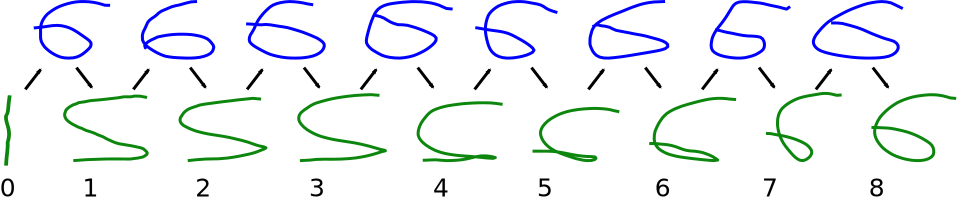
\includegraphics[width=0.9\linewidth]{learning_6_demos}
    \caption{\small Henry's demonstrations for the number ``6'' (top row) and
        corresponding shapes generated by the robot. After eight demonstrations,
        Henry decided that the robot's ``6'' was good enough, and went to
    another character: in that respect, he was the one leading the learning
process of the robot.}
    \label{learning_6_demos}
\end{figure}


\begin{figure}
    \centering
    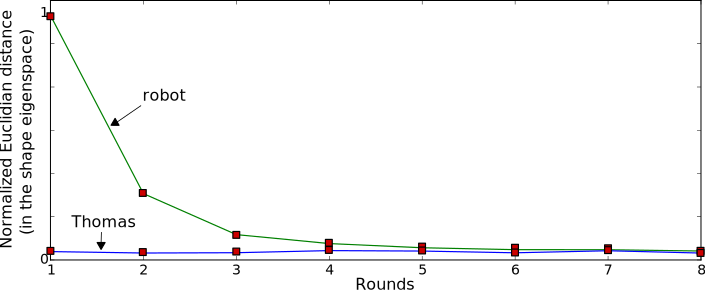
\includegraphics[width=0.9\linewidth]{learning_6_distances}
    \caption{\small Two metrics to assess the handwriting progresses: Euclidian
    distance in the eigenspace of the number dataset (top figure) or in
cartesian space (bottom figure). Green lines represent the robot performance,
blue lines Henry's performance. The round IDs correspond to the demonstrations
pictured on Figure~\ref{henry_demos}.}
    \label{henry_distances}
\end{figure}

%%%%%%%%%%%%%%%%%%%%%%%%%%%%%%%%%%%%%%%%%%%%%%%%%%%%%%%%%%%%%%%%%%%%%%%%%%%%%%%%%%%
%%%%%%%%%%%%%%%%%%%%%%%%%%%%%%%%%%%%%%%%%%%%%%%%%%%%%%%%%%%%%%%%%%%%%%%%%%%%%%%%%%%
\section{Conclusion}

The CoWriter project, as presented above, gives a novel perspective on educative
robots, at several levels:

\begin{itemize}
    \item robots in an educative context are \textbf{relevant and effective beyond ICT
        teaching},

    \item we can successfully \textbf{transpose the well-established
        \emph{learning by teaching} paradigm} from education sciences to
        robotics, even in a \textbf{complex form}: handwriting is difficult
        physical skill, the robot learns and interact autonomously, the child is
        responsible not only for the teaching but also for the teaching
        orchestration by managing the turn taking and the progression of the
        activity,

    \item blending machine-learning techniques with human-robot interaction
        allows for building a \textbf{believable agent}, that induces
        \textbf{social commitment},

    \item this proves essential to \textbf{sustain a long-term interaction} (several
        hours) around a fundamentally routine -- yet challenging -- educational
        task (hand-writing learning).
\end{itemize}


No surprisingly, the role of the robot \textit{vis-a-vis} the teacher has also
been questioned (including an angry email from one teacher: ``You want to
replace us!''): as we see it, the role of the robot within the classroom (or at
the therapist's surgery) does not infringe upon the role of the adult (teacher
or therapist).  The core of the \emph{learning by teaching} paradigm relies on
the child becoming the teacher of an underperforming pupil (the robot): from
that perspective, the robot does not replace the teacher, on the contrary. It
plays a different role in the classroom, which happen to be novel as well: the
robot is the \emph{least} performing student, and however a very patient, always
eager to improve, one.

The importance of the adult is further supported by our experiments: even with
an autonomous, nominally performing robot, to put the teacher's clothes on
remains (expectedly) difficult for 5-6 years old children, and during the
experiments we conducted, the adult always played a key role at prompting the
child to give feedback to the robot or to go to the next letter or word.  At a
higher orchestration level (and as reported in the two case studies with Diego
and Henry), the educational scenarios were also always designed and monitored by
the adults.

We initially envisioned the CoWriter system to be run in the back of a
classroom with one child: this would have allowed an individual, face-to-face
remediation approach, not otherwise tractable for a teacher with 20 pupils.
This is unlikely to happen. In our experience, the teacher keeps such an
important role that the interaction and the learning would hardly occur if the
child is left alone (or even semi-alone). At the end, we can reassure teachers:
robots are not going to replace them any time soon.

Beyond handwriting, we believe that this work provides a novel perspective on
the role for robots in the field of education. \emph{Learning by teaching} is a
powerful paradigm because of not only its pedagogical efficacy, but its
potential to positively impact the child's motivation and self-esteem. We hope that 
this article shows that this is a very relevant context of use for robots. Indeed,
when facing a child with school difficulties, robots can play the role of a na\"ive 
learner which neither adults nor peers -- because of the social effects it would 
induce -- can convincingly play.


%%%%%%%%%%%%%%%%%%%%%%%%%%%%%%%%%%%%%%%%%%%%%%%%%%%%%%%%%%%%%%%%%%%%%%%%%%%%%%%%%%%
%%%%%%%%%%%%%%%%%%%%%%%%%%%%%%%%%%%%%%%%%%%%%%%%%%%%%%%%%%%%%%%%%%%%%%%%%%%%%%%%%%%
\section*{Acknowledgments}

This research was partially supported by the Funda\c{c}\~{a}o para a Ci\^{e}ncia
e a Tecnologia (FCT) with reference UID/CEC/50021/2013, and by the Swiss
National Science Foundation through the National Centre of Competence in
Research Robotics.

\bibliographystyle{abbrv}
\bibliography{biblio}


\end{document}
